% ============================================================
%  presentacion_avances.tex
%  Avances metodológicos – Sesión de trabajo
%  Replicación: Carrillo & Elizondo (2015/2018)
% ============================================================
\documentclass[aspectratio=169, 10pt]{beamer}

% ── Tema y colores ──────────────────────────────────────────
\usetheme{Madrid}
\usecolortheme{seahorse}
\setbeamertemplate{navigation symbols}{}
\setbeamertemplate{footline}[frame number]

\definecolor{itamdark}{RGB}{110,15,25}
\definecolor{itamlight}{RGB}{200,160,160}
\definecolor{accentblue}{RGB}{31,119,180}
\definecolor{accentgreen}{RGB}{44,160,44}
\definecolor{accentred}{RGB}{214,39,40}
\setbeamercolor{frametitle}{bg=itamdark, fg=white}
\setbeamercolor{title}{fg=white}
\setbeamercolor{institute}{fg=itamlight}
\setbeamercolor{structure}{fg=itamdark}
\setbeamercolor{block title}{bg=itamdark!85, fg=white}
\setbeamercolor{block body}{bg=itamdark!8}
\setbeamercolor{alerted text}{fg=accentred}

% ── Paquetes ────────────────────────────────────────────────
\usepackage[utf8]{inputenc}
\usepackage[spanish]{babel}
\usepackage{booktabs}
\usepackage{multirow}
\usepackage{colortbl}
\usepackage{graphicx}
\usepackage{xcolor}
\usepackage{amsmath}
\usepackage{caption}
\captionsetup{font=scriptsize, labelformat=empty}
\graphicspath{{figures/}}

% ── Macros ──────────────────────────────────────────────────
\newcommand{\CE}{C\&E~(2015/18)}
\newcommand{\highlight}[1]{\textcolor{itamdark}{\textbf{#1}}}

% ── Portada ─────────────────────────────────────────────────
\title[Avances metodológicos]{Avances metodológicos en la replicación de\\
  Carrillo \& Elizondo (2015/2018)}
\subtitle{Brecha del producto $\cdot$ Pruebas ADF $\cdot$
          Identificación estructural $\cdot$ Diagnósticos del VAR}
\author{Carlos Varras}
\institute[ITAM]{Instituto Tecnológico Autónomo de México\\
  \smallskip Seminario de Investigación}
\date{Abril 2026}

% ============================================================
\begin{document}
% ============================================================

% ── Portada ─────────────────────────────────────────────────
{
\setbeamertemplate{footline}{}
\begin{frame}
  \titlepage
\end{frame}
}

% ── Índice ──────────────────────────────────────────────────
\begin{frame}{Agenda}
  \tableofcontents[hideallsubsections]
\end{frame}

% ============================================================
\section{Brecha del producto: Filtro de Kalman MFK}
% ============================================================

\begin{frame}{Brecha del producto — Modelo de Filtro de Kalman (MFK)}

  \begin{columns}[T]

    \column{0.52\textwidth}
    \textbf{\small Metodología (Elizondo, 2012)}
    \begin{itemize}\setlength\itemsep{4pt}
      \item[\highlight{1.}] El IGAE desestacionalizado (nivel, base 2018=100) sirve
            como \alert{observable} $Z_t = \Delta\log(\text{IGAE}_t)$
      \item[\highlight{2.}] El crecimiento mensual del PIB $X_t = \Delta\log(\text{PIB}_t)$
            es el \alert{estado no observable}
      \item[\highlight{3.}] Modelo espacio-estado:
        \begin{align*}
          X_t &= A\,X_{t-1} + w_t, \quad w_t \sim \mathcal{N}(0,Q) \\
          Z_t &= H\,X_t + v_t,\quad v_t \sim \mathcal{N}(0,R)
        \end{align*}
      \item[\highlight{4.}] Los cuatro parámetros $\{A,H,Q,R\}$ se estiman
            \textit{conjuntamente} por \alert{máxima verosimilitud}
            (filtro de Kalman dentro de la función de log-verosimilitud)
      \item[\highlight{5.}] El suavizado de Kalman entrega $\hat{X}_t$;
            el nivel mensual del PIB se reconstruye por
            \highlight{integración acumulada} anclada en el PIB trimestral de Q1-1993
      \item[\highlight{6.}] Se aplica filtro \alert{HP ($\lambda=129{,}600$)} sobre
            $\log\widehat{\text{PIB}}_t^{\text{mensual}}$;
            la brecha $= (\log\text{PIB} - \text{tendencia})\times 100$
    \end{itemize}

    \column{0.46\textwidth}
    \textbf{\small Parámetros estimados}
    \vspace{3pt}
    \begin{block}{}
      \centering\small
      \begin{tabular}{lrl}
        \toprule
        Parámetro & Valor & Interpretación \\
        \midrule
        $\hat{A}$ & $0.193$ & Persistencia AR del crec.\ PIB \\
        $\hat{H}$ & $1.000$ & Loading IGAE/PIB (restringido) \\
        $\hat{Q}$ & $0.000214$ & Varianza ruido de estado \\
        $\hat{R}$ & $\approx 0$ & Varianza ruido de medición \\
        \bottomrule
      \end{tabular}
    \end{block}
    \vspace{6pt}
    \textbf{\small Nota económica:} $\hat{H}=1$ y $\hat{R}\approx 0$ implican que el
    IGAE es un \textit{proxy} casi perfecto del PIB mensual en tasas de crecimiento
    — resultado consistente con la evidencia de Elizondo (2012) y con la
    construcción metodológica del IGAE por parte del INEGI.

  \end{columns}

\end{frame}

% ── Validación ──────────────────────────────────────────────
\begin{frame}{Brecha Kalman MFK — Validación comparativa}

  \begin{columns}[T]

    \column{0.48\textwidth}
    \textbf{\small Estadísticos descriptivos (Ene 2001 – Mar 2014)}
    \vspace{4pt}

    \begin{table}
      \centering\small
      \begin{tabular}{lcccc}
        \toprule
        Serie & $\bar{x}$ & $\hat{\sigma}$ & Mín & Máx \\
        \midrule
        \rowcolor{accentblue!15}
        Kalman MFK & $-0.305$ & $2.180$ & $-7.69$ & $3.54$ \\
        INEGI ex-petróleo & $-0.291$ & $2.138$ & $-7.25$ & $3.88$ \\
        Banxico (anterior) & $-0.263$ & $1.994$ & $-6.80$ & $3.40$ \\
        \bottomrule
      \end{tabular}
    \end{table}

    \vspace{5pt}
    \begin{block}{Correlaciones con la serie Kalman}
      \centering\small
      \begin{tabular}{lc}
        \toprule
        Serie & $\hat{\rho}$ \\
        \midrule
        INEGI ex-petróleo & $0.940$ \\
        Banxico original  & $0.940$ \\
        \bottomrule
      \end{tabular}
    \end{block}

    \vspace{5pt}
    \footnotesize
    \textbf{Conclusión:} Media y varianza son prácticamente idénticas entre la
    estimación Kalman y la serie INEGI ($\Delta\bar{x} < 0.02$,
    $\Delta\hat{\sigma} < 0.05$). La correlación de $0.94$ confirma equivalencia
    metodológica con mayor control sobre la construcción de la brecha.

    \column{0.50\textwidth}
    \textbf{\small Comparación de estimaciones}
    \vspace{2pt}
    \begin{center}
      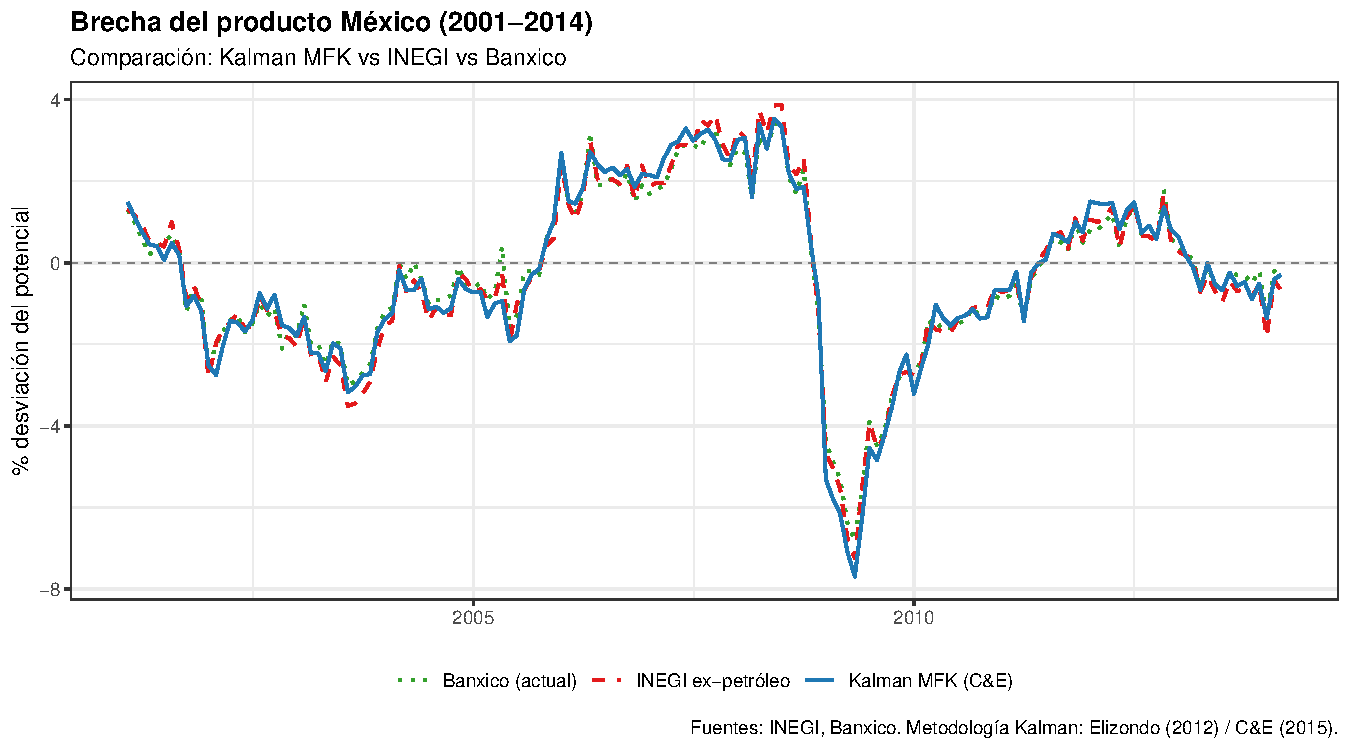
\includegraphics[width=\linewidth]{brecha_kalman_comparacion.pdf}
    \end{center}

    \vspace{2pt}
    \textbf{\small Series detrended — VAR (Fig.\ 6 equivalente)}
    \vspace{2pt}
    \begin{center}
      \includegraphics[width=\linewidth, height=2.8cm, keepaspectratio]%
        {fig_series_gaps.png}
    \end{center}

  \end{columns}

\end{frame}

% ============================================================
\section{Prueba ADF — Raíz unitaria}
% ============================================================

\begin{frame}{Prueba ADF — Resolución de la estacionariedad}

  \begin{columns}[T]

    \column{0.50\textwidth}
    \textbf{\small Problema: especificación incorrecta del test}
    \vspace{3pt}
    \begin{itemize}\setlength\itemsep{4pt}
      \item La implementación original usaba \texttt{adf.test(x, k=3)} de
            \texttt{tseries}: número fijo de rezagos e inclusión automática de
            tendencia y constante para todas las variables
      \item Con $k=1{-}3$, los \alert{residuos del ADF presentan autocorrelación
            serial} (Ljung-Box $p<0.05$) para \texttt{igae} y \texttt{y\_us\_gap}
            $\Rightarrow$ test \textbf{inválido}: sesga hacia no rechazar $H_0$
    \end{itemize}

    \vspace{4pt}
    \textbf{\small Solución: selección adaptativa de rezagos}
    \vspace{3pt}
    \begin{block}{Criterio LB-adaptativo}
      Mínimo $k \in [1, k_{\max}]$ tal que $\text{LB}(12)\; p > 0.10$
      (residuos blancos). $k_{\max} = \max(\lfloor(n-1)^{1/3}\rfloor, 5)$.
    \end{block}

    \vspace{4pt}
    \begin{itemize}\setlength\itemsep{4pt}
      \item \texttt{igae}, \texttt{y\_us\_gap}: requieren $k=4$ (alta
            persistencia near-$I(1)$); con $k<4$ los residuos del ADF
            están autocorrelacionados
      \item \texttt{i\_gap}: $k=1$ es suficiente; más rezagos
            reintroducen autocorrelación (estructura ARMA del diferencial de tasas)
    \end{itemize}

    \column{0.48\textwidth}
    \textbf{\small Resultado: todas las variables son $I(0)$}
    \vspace{4pt}

    \begin{center}
      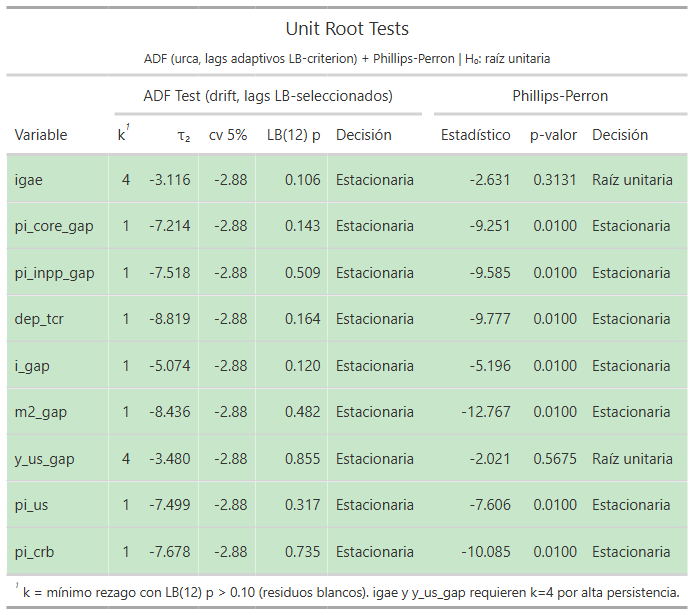
\includegraphics[width=\linewidth]{tabla_adf_pp.png}
    \end{center}

    \vspace{4pt}
    \footnotesize
    \textbf{Consistencia con \CE:} el paper reporta estacionariedad para todas
    las variables (Apéndice C). La discrepancia en la implementación previa no
    era una limitación de los datos, sino de la selección de rezagos del test.
    Con el criterio LB-adaptativo los resultados son plenamente consistentes.

  \end{columns}

\end{frame}

% ============================================================
\section{Restricciones de signo — Distribución de Haar}
% ============================================================

\begin{frame}{Restricciones de signo — Consistencia con \CE\ y la literatura}

  \begin{columns}[T]

    \column{0.50\textwidth}
    \textbf{\small El algoritmo (Rubio-Ramírez et al., 2010)}
    \vspace{3pt}
    \begin{enumerate}\setlength\itemsep{5pt}
      \item[\textbf{[1]}] Factorización de Cholesky $\mathbf{P}$ de $\hat{\Sigma}_u$
      \item[\textbf{[2]}] Generar $\mathbf{Q}$ ortogonal aleatoria
            ($\mathbf{Q} \sim \text{Haar sobre } O(n)$)
      \item[\textbf{[3]}] Candidato: $\mathbf{B} = \mathbf{P}\mathbf{Q}$;
            calcular efectos de impacto
            $\mathbf{b}_j = \mathbf{B}_{:,j}$ (columna $j = i_{gap}$)
      \item[\textbf{[4]}] ¿Restricciones de signo satisfechas (Tabla 2)?
        \begin{itemize}
          \item Sí $\to$ almacenar $\mathbf{B}$; regresar a [2]
          \item No $\to$ descartar; regresar a [2]
        \end{itemize}
    \end{enumerate}

    \vspace{6pt}
    \textbf{\small ¿Por qué la medida de Haar?}
    \begin{itemize}\setlength\itemsep{3pt}
      \item \alert{Única} medida de probabilidad invariante bajo
            transformaciones ortogonales sobre $O(n)$: el ``uniforme''
            del grupo de rotaciones
      \item Garantiza que la búsqueda no favorece \textit{a priori}
            ninguna dirección de rotación $\to$ inferencia no sesgada
            sobre el conjunto identificado
      \item Se genera vía QR de una matriz aleatoria + corrección de
            signo de la diagonal de $R$
    \end{itemize}

    \column{0.48\textwidth}
    \textbf{\small ¿Por qué es correcto?}
    \vspace{3pt}
    \begin{block}{Identidad algebraica clave}
      $\mathbf{B}\mathbf{B}^\top = \mathbf{P}\underbrace{\mathbf{Q}\mathbf{Q}^\top}_{=\,\mathbf{I}}\mathbf{P}^\top
      = \hat{\Sigma}_u$
    \end{block}
    \vspace{4pt}
    \begin{itemize}\setlength\itemsep{5pt}
      \item La ortogonalidad de $\mathbf{Q}$ preserva la factorización
            de $\hat{\Sigma}_u$ $\Rightarrow$ $\mathbf{B}$ es siempre
            una descomposición estructural válida
      \item Forzar signos multiplicando por $\text{diag}(\pm 1)$
            \alert{sesga la distribución posterior} implícita de $\mathbf{B}$
            y viola la identificación de conjunto
      \item Nuestro MATLAB: rechazo puro (Haar + accept/reject),
            \textbf{idéntico al Algoritmo 1 de \CE}
    \end{itemize}

    \vspace{4pt}
    \begin{center}
      \includegraphics[width=\linewidth, height=3.0cm, keepaspectratio]%
        {fig8_sign_restrictions.png}
    \end{center}
    {\fontsize{7}{8.5}\selectfont
      \textit{Figura 8: Standard (fila sup.) y Augmented (fila inf.).
      2\,000 bootstraps $\times$ 4 modelos.}}

  \end{columns}

\end{frame}

% ============================================================
\section{Diagnósticos del VAR — Estadístico PT}
% ============================================================

\begin{frame}{Autocorrelación en residuos del VAR — Test de Portmanteau}

  \begin{columns}[T]

    \column{0.50\textwidth}
    \textbf{\small Estadístico PT (sistema) vs.\ Ljung-Box por ecuación}
    \vspace{3pt}
    \begin{itemize}\setlength\itemsep{4pt}
      \item El PT de \texttt{serial.test} evalúa la matriz completa de
            autocorrelaciones cruzadas ($n^2 \times h$ momentos);
            \alert{una sola ecuación con persistencia contamina el sistema}
      \item Para $h \leq p = 3$: los grados de libertad $n^2(h-p) \leq 0$
            $\Rightarrow$ el test \textbf{no está definido}
            (produce \texttt{NaN} en R)
      \item Solución: \alert{Ljung-Box ecuación por ecuación}
            sobre los residuos de cada variable individualmente
    \end{itemize}

    \vspace{5pt}
    \begin{block}{Resultado clave}
      Con la brecha Kalman, \textbf{ninguna ecuación rechaza $H_0$} al 5\%
      para $h = 3, 6, 12$. Mejora sobre \CE, que reporta rechazo en
      output gap usando la serie Banxico original.
    \end{block}

    \vspace{5pt}
    \footnotesize
    \textbf{Por qué no invalida el modelo:} el bootstrap de Runkle (1987)
    remuestrea los residuos tal como son, sin suponer i.i.d.\ La
    identificación (Cholesky y restricciones de signo) solo requiere
    que la descomposición de $\hat{\Sigma}_u$ sea consistente.

    \column{0.48\textwidth}
    \textbf{\small Ljung-Box por ecuación — VAR(3) con exógenas}
    \vspace{3pt}

    \begin{table}
      \centering
      {\fontsize{7.5}{9.5}\selectfont
      \begin{tabular}{lcccccc}
        \toprule
        & \multicolumn{2}{c}{$h=3$} & \multicolumn{2}{c}{$h=6$}
        & \multicolumn{2}{c}{$h=12$} \\
        \cmidrule(lr){2-3}\cmidrule(lr){4-5}\cmidrule(lr){6-7}
        Variable & $Q$ & $p$ & $Q$ & $p$ & $Q$ & $p$ \\
        \midrule
        Output gap         & 2.23 & .526 &  7.47 & .279 & 16.63 & .164 \\
        Inflation (core)   & 0.46 & .928 &  0.49 & .998 &  5.46 & .941 \\
        PPI                & 0.13 & .988 &  1.29 & .972 &  9.95 & .620 \\
        Real ER dep.       & 0.10 & .992 &  2.21 & .899 &  9.85 & .629 \\
        Nom.\ interest rate & 0.72 & .867 &  8.44 & .207 & 19.44 & .078 \\
        Money growth       & 1.54 & .673 &  6.30 & .390 & 11.58 & .480 \\
        \midrule
        \multicolumn{7}{l}{\cellcolor{accentgreen!25}%
          \footnotesize\textbf{Ningún $p < 0.05$}
          $\Rightarrow$ No se rechaza $H_0$ en ninguna ecuación} \\
        \bottomrule
      \end{tabular}}
      \caption*{\footnotesize $H_0$: sin autocorrelación serial hasta $h$.
                Muestra: Feb 2001 – Mar 2014 ($T=155$).}
    \end{table}

    \vspace{2pt}
    \footnotesize
    \textbf{Comparación con \CE:} reportan rechazo en output gap
    ($Q(3)\approx 8.7$, $p{<}0.05$) con la serie Banxico.
    La brecha Kalman reduce esa persistencia residual ($Q(3){=}2.23$,
    $p{=}0.53$) — el cambio de serie efectivamente resuelve el problema.

  \end{columns}

\end{frame}

% ============================================================
\section{Funciones impulso-respuesta}
% ============================================================

\begin{frame}{Funciones impulso-respuesta — Los tres esquemas de identificación}

  \begin{columns}[T]

    \column{0.33\textwidth}
    \textbf{\small Fig.\ 7 — Exclusión (Cholesky)}
    \vspace{2pt}
    \begin{center}
      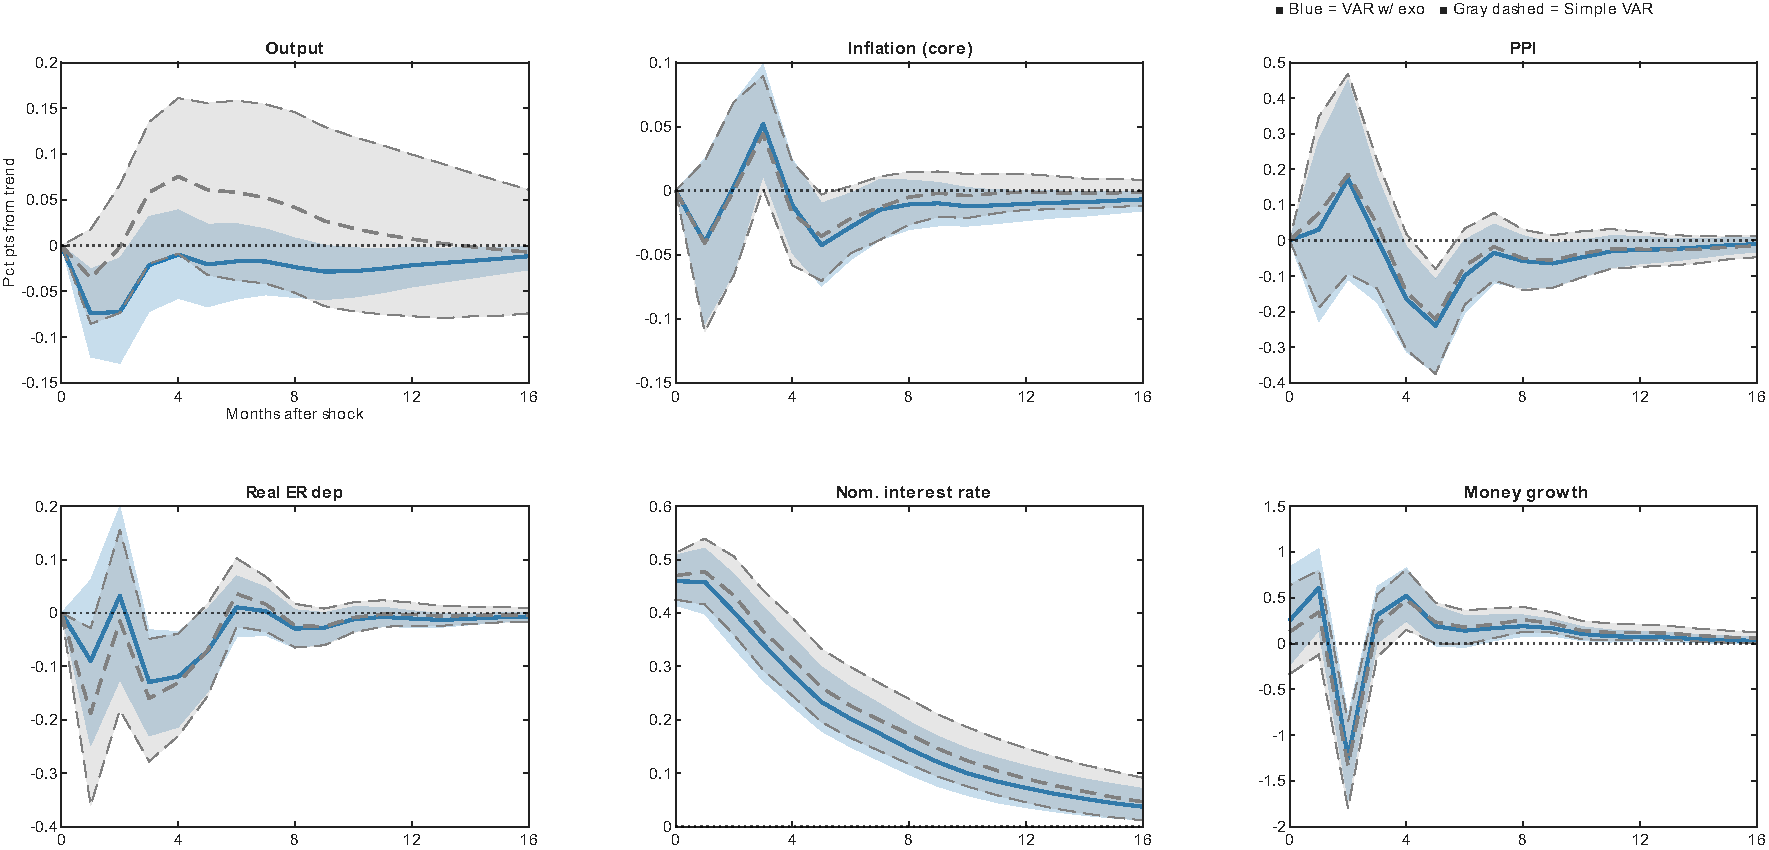
\includegraphics[width=\linewidth]{fig7_exclusion.pdf}
    \end{center}
    \vspace{2pt}
    {\fontsize{7.5}{9}\selectfont
    Choque contractivo en $i_{gap}$: VAR con bloque exógeno
    (azul) $\to$ caída del output y deflación
    \textit{hump-shaped} (${\approx}6$ meses).
    VAR simple (gris) no descarta \textit{price puzzle}.}

    \column{0.33\textwidth}
    \textbf{\small Fig.\ 8 — Restricciones de signo}
    \vspace{2pt}
    \begin{center}
      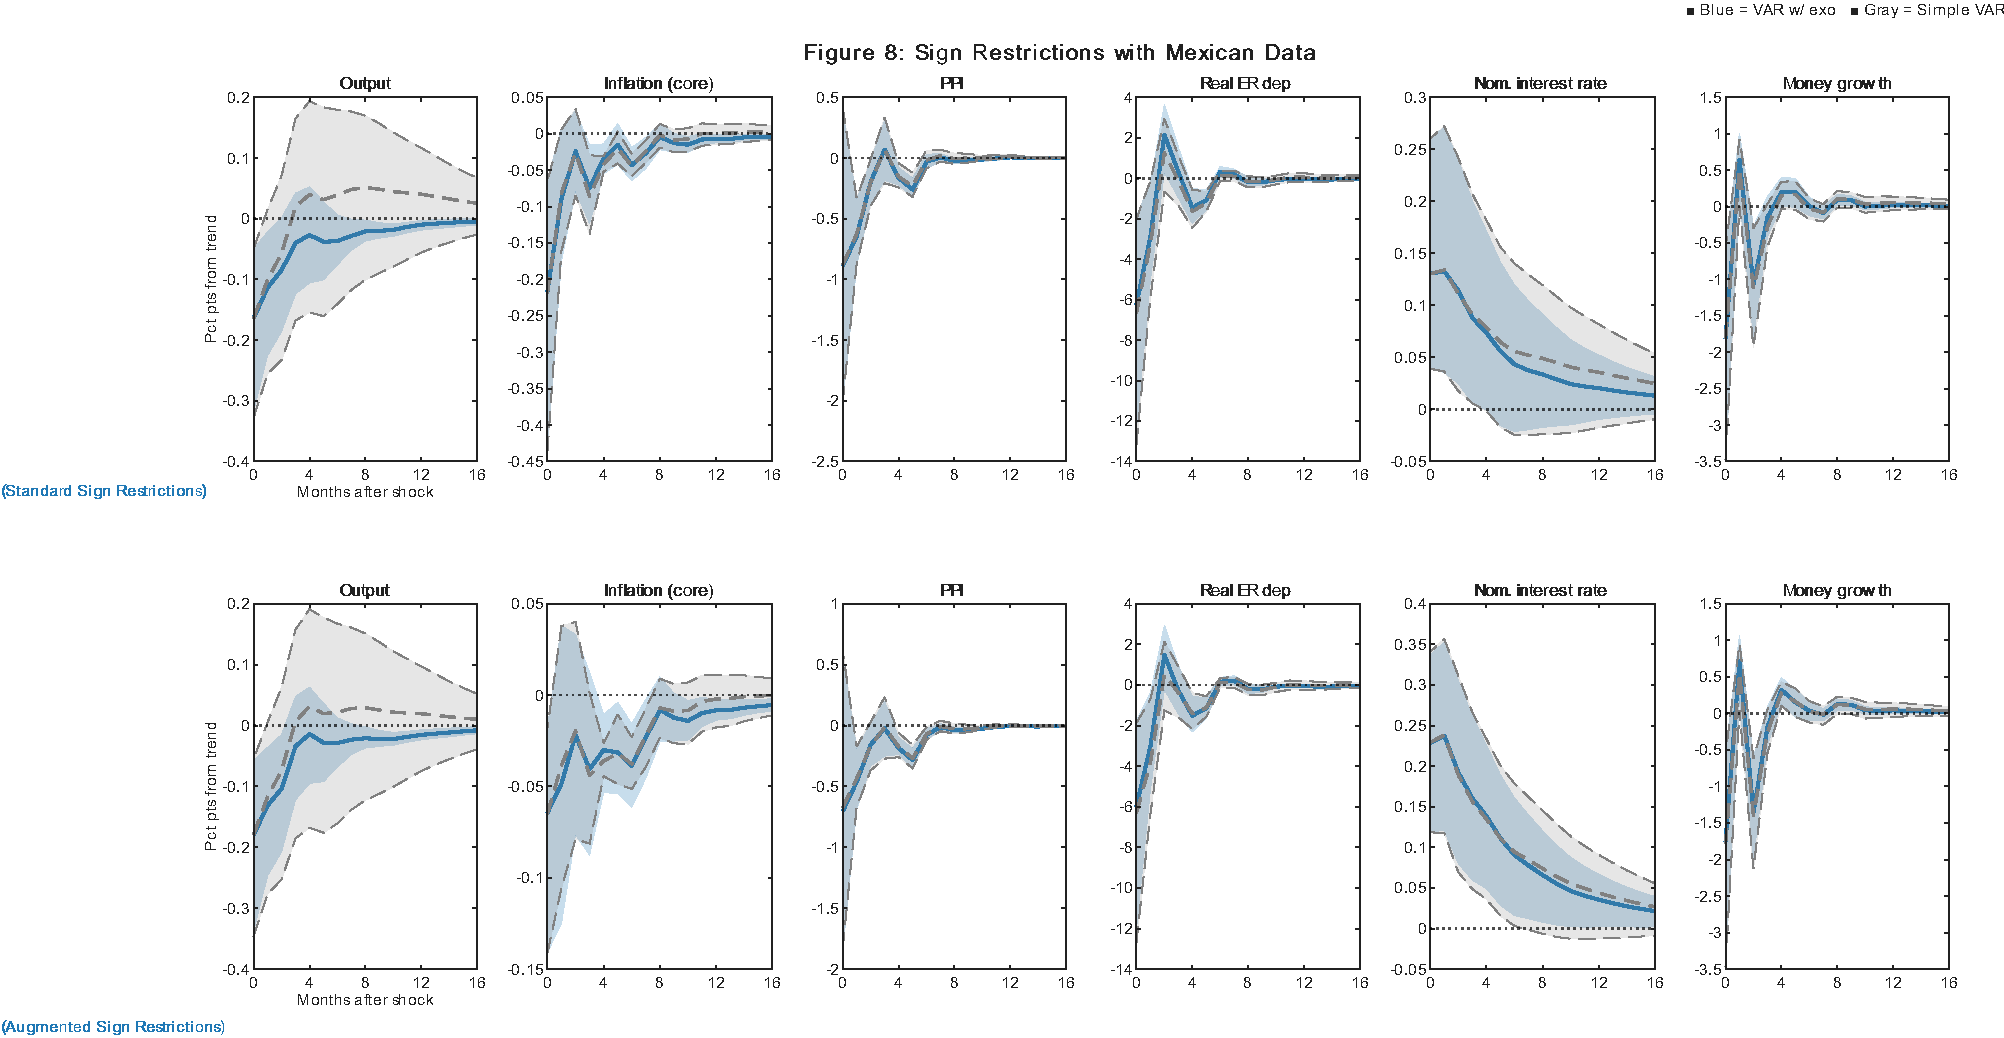
\includegraphics[width=\linewidth]{fig8_sign_restrictions.pdf}
    \end{center}
    \vspace{2pt}
    {\fontsize{7.5}{9}\selectfont
    Restricciones aumentadas reducen la respuesta de impacto
    de inflación de $-2.5$ a $-0.06$ pp y eliminan el
    \textit{price puzzle} con mayor probabilidad.}

    \column{0.33\textwidth}
    \textbf{\small Fig.\ 9 — Comparación de estrategias}
    \vspace{2pt}
    \begin{center}
      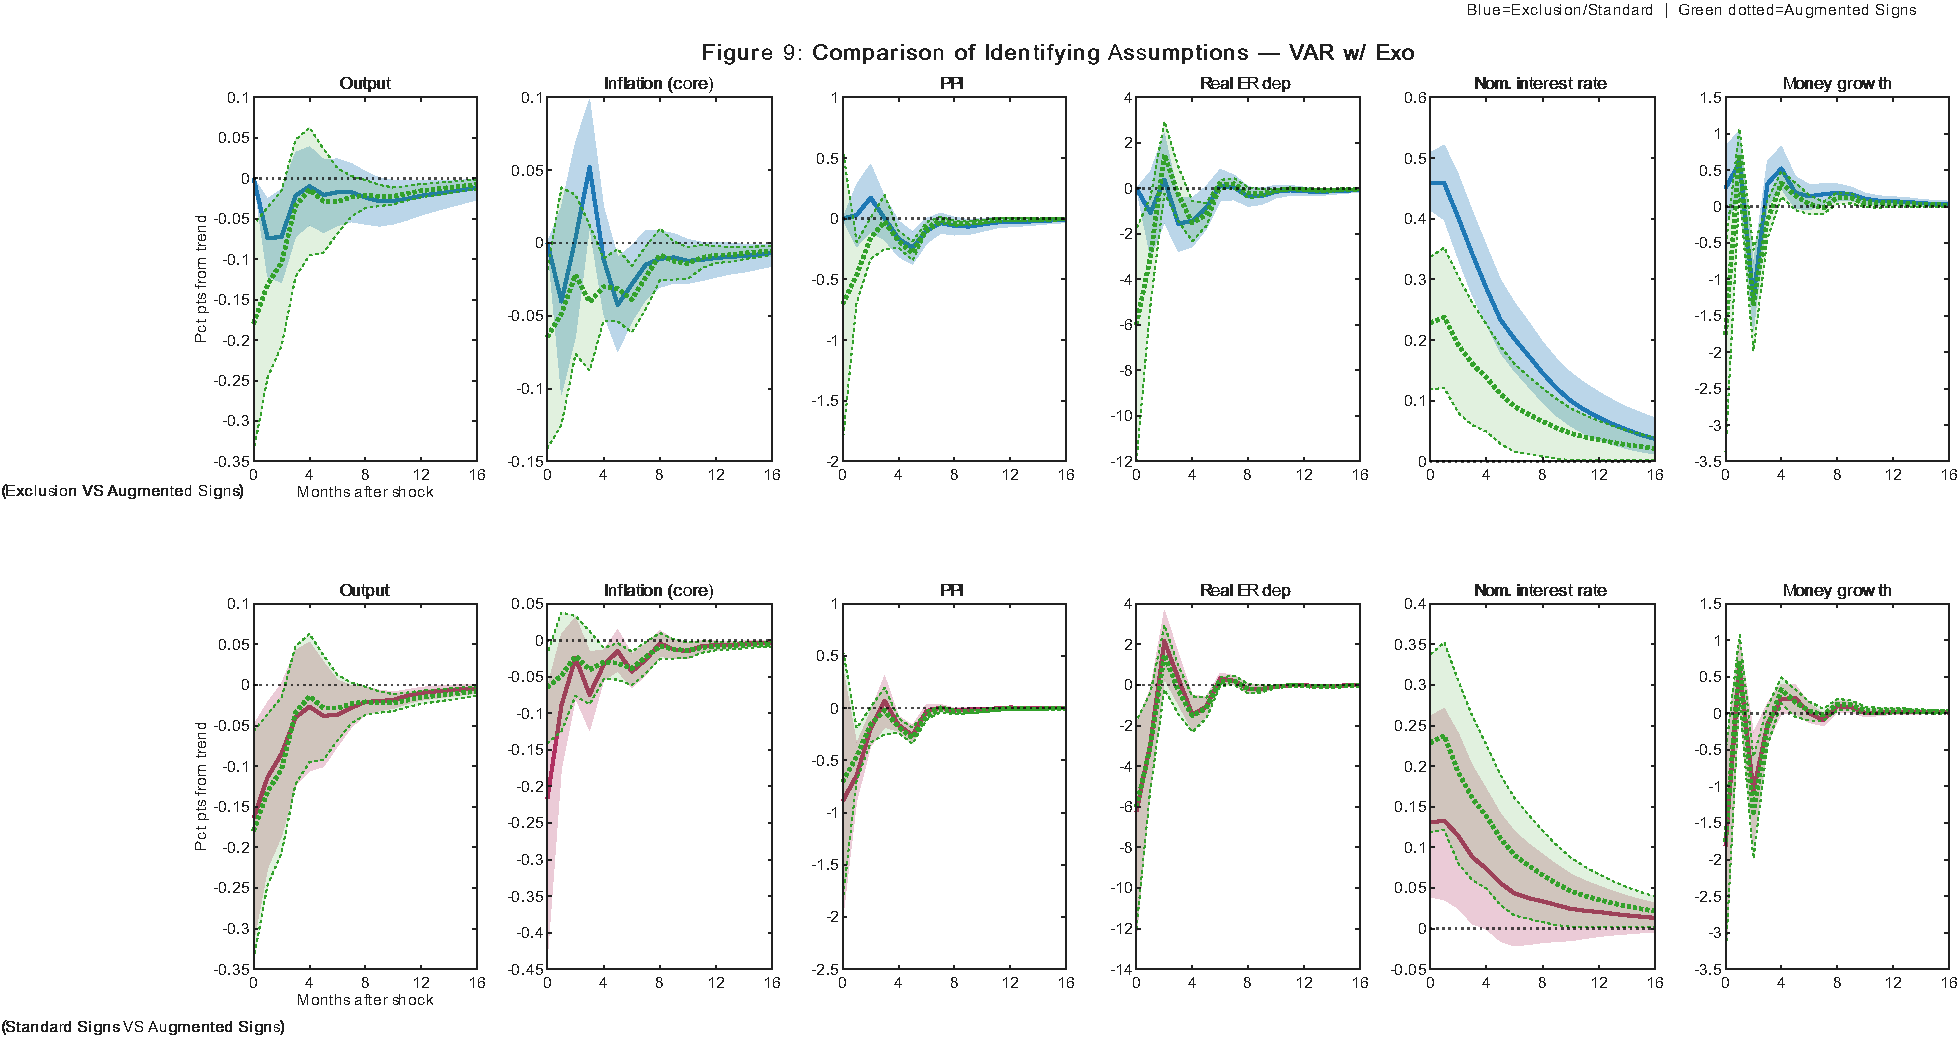
\includegraphics[width=\linewidth]{fig9_comparison.pdf}
    \end{center}
    \vspace{2pt}
    {\fontsize{7.5}{9}\selectfont
    Las tres estrategias producen IRFs cualitativamente
    consistentes. La identificación aumentada concentra
    la masa en estimaciones más precisas (bandas 68\% más angostas).}

  \end{columns}

\end{frame}

% ============================================================
%  APÉNDICE
% ============================================================
\appendix
\setbeamertemplate{footline}[text line]{\hfill\footnotesize Apéndice}

\begin{frame}{Apéndice — Resumen de decisiones metodológicas}

  \begin{table}
    \centering\small
    \begin{tabular}{p{3.0cm}p{5.4cm}p{4.8cm}}
      \toprule
      \textbf{Elemento} & \textbf{Paper \CE} & \textbf{Replicación} \\
      \midrule
      Brecha del producto
        & IGAE Banxico (precalculada)
        & Kalman MFK propio (Elizondo 2012) \\
      Similitud con paper
        & ---
        & $\hat{\rho} = 0.94$, $\Delta\bar{x}<0.02$, $\Delta\hat{\sigma}<0.05$ \\
      Test ADF
        & Todas $I(0)$, espec.\ no reportada
        & Urca + LB-adaptativo, todas $I(0)^{**}$ \\
      LB residuos
        & Output gap rechaza $H_0$
        & Ninguna ecuación rechaza $H_0$ al 5\% \\
      Identificación sign
        & Haar + accept/reject
        & Idéntico (Algoritmo 1) \\
      Bootstrap
        & Runkle (1987), 2\,000 réplicas
        & Idéntico \\
      Bandas de IC
        & 68\% (percentiles 16–84)
        & Idéntico \\
      $\beta_{\text{lower}}$
        & $-0.7$ (IC 95\% one-sided)
        & $-0.715$ (HAC Newey-West, lag=3) \\
      \bottomrule
    \end{tabular}
  \end{table}

\end{frame}

% ============================================================
\end{document}
% ============================================================
